\documentclass{tufte-handout}

\title{One-Way ANOVA with Repeated Measures}

%\author[The Tufte-LaTeX Developers]{The Tufte-\LaTeX\ Developers}

\date{} % without \date command, current date is supplied


\usepackage{graphicx} % allow embedded images
  \setkeys{Gin}{width=\linewidth,totalheight=\textheight,keepaspectratio}
  \graphicspath{{graphics/}} % set of paths to search for images
\usepackage{amsmath}  % extended mathematics
\usepackage{booktabs} % book-quality tables
\usepackage{units}    % non-stacked fractions and better unit spacing
\usepackage{multicol} % multiple column layout facilities
\usepackage{lipsum}   % filler text
\usepackage{fancyvrb} % extended verbatim environments
  \fvset{fontsize=\normalsize}% default font size for fancy-verbatim environments

\usepackage{pgfplots}
\pgfplotsset{compat=1.12}

% Standardize command font styles and environments
\newcommand{\doccmd}[1]{\texttt{\textbackslash#1}}% command name -- adds backslash automatically
\newcommand{\docopt}[1]{\ensuremath{\langle}\textrm{\textit{#1}}\ensuremath{\rangle}}% optional command argument
\newcommand{\docarg}[1]{\textrm{\textit{#1}}}% (required) command argument
\newcommand{\docenv}[1]{\textsf{#1}}% environment name
\newcommand{\docpkg}[1]{\texttt{#1}}% package name
\newcommand{\doccls}[1]{\texttt{#1}}% document class name
\newcommand{\docclsopt}[1]{\texttt{#1}}% document class option name
\newenvironment{docspec}{\begin{quote}\noindent}{\end{quote}}% command specification environment


\begin{document}

\maketitle% this prints the handout title, author, and date


%\printclassoptions


\begin{marginfigure}[50pt]
  \includegraphics[width=\linewidth]{anova_partition_one_way_repeat}%
  \label{fig:fullfig}%
  \setfloatalignment{t}
  \caption{Partitioning the Sum of Squares for the One-Way ANOVA with Repeated Measures}
\end{marginfigure}

\begin{marginfigure}[50pt]
  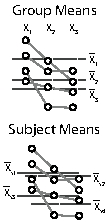
\includegraphics[width=\linewidth]{handout5_repeated}%
  \label{fig:fullfig}%
  \setfloatalignment{t}
  \caption{With repeated measures anova, we control for individual differences by using the mean for each subject.}
\end{marginfigure}

Suppose we wish to determine whether a set of sample means ($\bar{X}_1,\bar{X}_2,\cdots$) show a statistically significant difference when the samples are dependent. Similar to the one-way ANOVA with independent measures, for a one-way ANOVA with \emph{repeated measures} from $k$  groups we want to quantify variability between groups and variability within groups. However, with repeated measures, we can now attribute some of the within groups variability to individual differences! Rather than using "within groups" variability in the denominator we will use "error" variability:

\begin{align*}
&F=\frac{SS_{\text{between groups}}/df_{\text{between groups}}}{SS_{\text{error}}/df_{\text{error}}} & &\\
&SS_{\text{between groups}}=\sum_{\text{groups}} n_i(\bar{X}_i-\bar{X}_{\text{All}})^2 & &df_{\text{between groups}}=k-1\\
&SS_{\text{within groups}} =\sum_{\text{groups}} \sum_{\text{scores}} (X-\bar{X}_i)^2  & &df_{\text{within groups}}=N-k\\
&SS_{\text{between subjects}} = k \sum_{\text{subjects}} (\bar{X}_{s}-\bar{X}_{\text{All}})^2 & &df_{\text{between subjects}}=n-1\\
&SS_{\text{error}} = SS_{\text{within groups}} - SS_{\text{between subjects}}& &df_{\text{error}}=(n-1)(k-1)
\end{align*}

The notation is as before, but now we also have "subject means" $\bar{X}_s$. Just like the independent measures ANOVA, we can take advantage of the fact that variability can be "partitioned" to make the calculations easier. Here we have two levels of partitioning: first, the total variability, which is exactly as it was partitioned before $\dots$
\begin{align*}
&SS_{\text{total}}=\sum (X-\bar{X}_{\text{All}})^2\\
&SS_{\text{total}}=SS_{\text{between groups}} + SS_{\text{within groups}}\\
&df_{\text{total}}=df_{\text{between groups}} + df_{\text{within groups}}=N-1
\end{align*}
Then as the second level, we further partition the "within groups" variability...
\begin{align*}
&SS_{\text{within groups}}=SS_{\text{between subjects}} + SS_{\text{error}}\\
&df_{\text{within groups}}=df_{\text{between subjects}} + df_{\text{error}}
\end{align*}

Finally, the effect size, Variance Accounted For, with the repeated measures ANOVA also has the individual differences removed

\begin{equation*}
\eta^2 = \frac{SS_{\text{between groups}}}{SS_{\text{between groups}}+SS_{\text{error}}}
\end{equation*}

\pagebreak
\section{Example}

\begin{fullwidth}
Suppose you collect data using a repeated-measures design with 5 participants in three different conditions, and observe the data below. What is the value for the test statistic $F$?

\begin{table}
  \centering
  \fontfamily{ppl}\selectfont
  \begin{tabular}{rcccc}
    \toprule
    & Condition 1 & Condition 2 & Condition 3 & $\bar{X}_s$\\
    \midrule
Subject 1&	5&	2&	2&\\
Subject 2&	4&	2&	3&\\
Subject 3&	7&	3&	5&\\
Subject 4&	4&	2&	3&\\
Subject 5&	0&	1&	2&\\
\midrule
$\bar{X}=$&&&\\
$SS=$&&&\\
    \bottomrule
  \end{tabular}
  \label{tab:normaltab}
  %\zsavepos{pos:normaltab}
\end{table}

\vspace{4.25 in}

\begin{table}
  \centering
  \fontfamily{ppl}\selectfont
  \begin{tabular}{lllll}
    \toprule
    Source & \qquad SS & \qquad df & \qquad MS & \qquad F \\
    \midrule
    Between Groups & & & & \\
    Within Groups & & & & \\
\qquad Between Subjects & & & & \\
\qquad Error & & & & \\
    Total & & & & \\
    \bottomrule
  \end{tabular}
  \label{tab:normaltab}
  %\zsavepos{pos:normaltab}
\end{table}
\end{fullwidth}

\pagebreak
\section{Solution}

\begin{fullwidth}
\begin{table}
  \centering
  \fontfamily{ppl}\selectfont
  \begin{tabular}{rcccc}
    \toprule
    & Condition 1 & Condition 2 & Condition 3 & $\bar{X}_s$\\
    \midrule
Subject 1&	5&	2&	2&3\\
Subject 2&	4&	2&	3&3\\
Subject 3&	7&	3&	5&5\\
Subject 4&	4&	2&	3&3\\
Subject 5&	0&	1&	2&1\\
\midrule
$\bar{X}=$&4&2&3&\\
$SS=$&26&2&6&\\
    \bottomrule
  \end{tabular}
  \label{tab:normaltab}
  %\zsavepos{pos:normaltab}
\end{table}
\vspace{10pt}
Let's start by figurout out $SS_{\text{between groups}}$. From the table, we see we have $n=5$ subjects so $N=kn=3\cdot5=15$. After calculating the group means, the one thing we are missing is the "grand mean" $\bar{X}_{\text{All}}=(5+4+7+\cdots)/15=3$
Now we can fill in
\begin{align*}
&SS_{\text{between groups}}=\sum_{\text{groups}} n_i(\bar{X}_i-\bar{X}_{\text{All}})^2=5(4-3)^2+5(2-3)^2+5(3-3)^2=10\\
&df_{\text{between groups}}=k-1=3-1=2
\end{align*}
Now let's figure out $SS_{\text{within groups}}$
\begin{align*}
&SS_{\text{within groups}} =\sum_{\text{groups}} \sum_{\text{scores}} (X-\bar{X}_i)^2 = \sum_{\text{groups}} SS_i = 26+2+6=34\\
&df_{\text{within groups}} =N-k=15-3=12
\end{align*}
Now let's figure out $SS_{\text{between subjects}}$
\begin{align*}
&SS_{\text{between subjects}} = k \sum_{\text{subjects}} (\bar{X}_{s}-\bar{X}_{\text{All}})^2=3[(3-3)^2+(3-3)^2+(5-3)^2+(3-3)^2+(1-3)^2]=3[8]=24\\
&df_{\text{between groups}}=n-1=5-1=4
\end{align*}
Finally, to figure out $SS_\text{error}$, we'll use the formulas for partitioning the sum of squares $\dots$
\begin{align*}
&SS_{\text{error}}=SS_{\text{within groups}} - SS_{\text{between subjects}}=34-24=10\\
&df_{\text{error}}=(n-1)(k-1)=(5-1)(3-1)=(4)(2)=8
\end{align*}
\begin{table}
  \centering
  \fontfamily{ppl}\selectfont
  \begin{tabular}{lllll}
    \toprule
    Source &  SS &  df &  MS &  F \\
    \midrule
    Between Groups & 10 & 2 &5 &F=4 \\
    Within Groups & 34&12 & & \\
\qquad Between Subjects & 24&4 & & \\
\qquad Error & 10& 8 &1.25 & \\
    Total & 44&14 & & \\
    \bottomrule
  \end{tabular}
  \label{tab:normaltab}
  %\zsavepos{pos:normaltab}
\end{table}


\end{fullwidth}

\end{document}
